% Created by tikzDevice version 0.12.4 on 2023-11-07 14:08:56
% !TEX encoding = UTF-8 Unicode
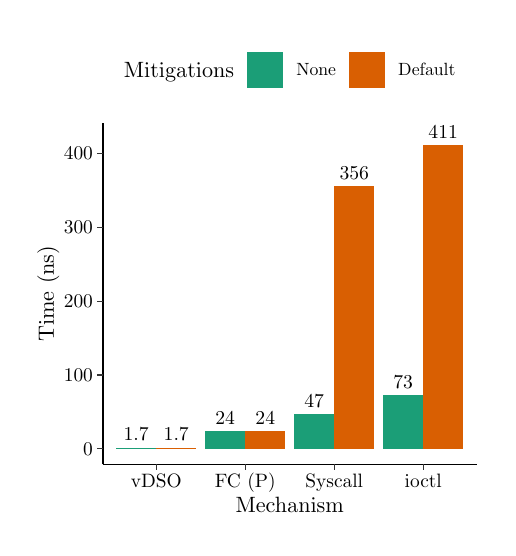
\begin{tikzpicture}[x=1pt,y=1pt]
\definecolor{fillColor}{RGB}{255,255,255}
\path[use as bounding box,fill=fillColor,fill opacity=0.00] (0,0) rectangle (166.22,180.67);
\begin{scope}
\path[clip] (  0.00,  0.00) rectangle (166.22,180.67);
\definecolor{drawColor}{RGB}{255,255,255}
\definecolor{fillColor}{RGB}{255,255,255}

\path[draw=drawColor,line width= 0.4pt,line join=round,line cap=round,fill=fillColor] (  0.00, -0.00) rectangle (166.22,180.67);
\end{scope}
\begin{scope}
\path[clip] ( 27.16, 22.85) rectangle (162.22,146.22);
\definecolor{fillColor}{RGB}{255,255,255}

\path[fill=fillColor] ( 27.16, 22.85) rectangle (162.22,146.22);
\definecolor{fillColor}{RGB}{27,158,119}

\path[fill=fillColor] ( 96.30, 28.45) rectangle (110.77, 41.01);
\definecolor{fillColor}{RGB}{217,95,2}

\path[fill=fillColor] (110.77, 28.45) rectangle (125.24,123.52);

\path[fill=fillColor] (142.93, 28.45) rectangle (157.40,138.21);

\path[fill=fillColor] ( 78.61, 28.45) rectangle ( 93.08, 34.86);

\path[fill=fillColor] ( 46.46, 28.45) rectangle ( 60.93, 28.91);
\definecolor{fillColor}{RGB}{27,158,119}

\path[fill=fillColor] (128.46, 28.45) rectangle (142.93, 47.95);

\path[fill=fillColor] ( 64.14, 28.45) rectangle ( 78.61, 34.86);

\path[fill=fillColor] ( 31.99, 28.45) rectangle ( 46.46, 28.91);
\definecolor{drawColor}{RGB}{0,0,0}

\node[text=drawColor,anchor=base,inner sep=0pt, outer sep=0pt, scale=  0.71] at (103.53, 43.46) {47};

\node[text=drawColor,anchor=base,inner sep=0pt, outer sep=0pt, scale=  0.71] at (118.01,125.97) {356};

\node[text=drawColor,anchor=base,inner sep=0pt, outer sep=0pt, scale=  0.71] at (150.16,140.66) {411};

\node[text=drawColor,anchor=base,inner sep=0pt, outer sep=0pt, scale=  0.71] at ( 85.85, 37.31) {24};

\node[text=drawColor,anchor=base,inner sep=0pt, outer sep=0pt, scale=  0.71] at ( 53.69, 31.36) {1.7};

\node[text=drawColor,anchor=base,inner sep=0pt, outer sep=0pt, scale=  0.71] at (135.69, 50.40) {73};

\node[text=drawColor,anchor=base,inner sep=0pt, outer sep=0pt, scale=  0.71] at ( 71.38, 37.31) {24};

\node[text=drawColor,anchor=base,inner sep=0pt, outer sep=0pt, scale=  0.71] at ( 39.22, 31.36) {1.7};
\end{scope}
\begin{scope}
\path[clip] (  0.00,  0.00) rectangle (166.22,180.67);
\definecolor{drawColor}{RGB}{0,0,0}

\path[draw=drawColor,line width= 0.6pt,line join=round] ( 27.16, 22.85) --
	( 27.16,146.22);
\end{scope}
\begin{scope}
\path[clip] (  0.00,  0.00) rectangle (166.22,180.67);
\definecolor{drawColor}{RGB}{0,0,0}

\node[text=drawColor,anchor=base east,inner sep=0pt, outer sep=0pt, scale=  0.70] at ( 23.56, 26.04) {0};

\node[text=drawColor,anchor=base east,inner sep=0pt, outer sep=0pt, scale=  0.70] at ( 23.56, 52.75) {100};

\node[text=drawColor,anchor=base east,inner sep=0pt, outer sep=0pt, scale=  0.70] at ( 23.56, 79.45) {200};

\node[text=drawColor,anchor=base east,inner sep=0pt, outer sep=0pt, scale=  0.70] at ( 23.56,106.16) {300};

\node[text=drawColor,anchor=base east,inner sep=0pt, outer sep=0pt, scale=  0.70] at ( 23.56,132.86) {400};
\end{scope}
\begin{scope}
\path[clip] (  0.00,  0.00) rectangle (166.22,180.67);
\definecolor{drawColor}{gray}{0.20}

\path[draw=drawColor,line width= 0.4pt,line join=round] ( 25.16, 28.45) --
	( 27.16, 28.45);

\path[draw=drawColor,line width= 0.4pt,line join=round] ( 25.16, 55.16) --
	( 27.16, 55.16);

\path[draw=drawColor,line width= 0.4pt,line join=round] ( 25.16, 81.86) --
	( 27.16, 81.86);

\path[draw=drawColor,line width= 0.4pt,line join=round] ( 25.16,108.57) --
	( 27.16,108.57);

\path[draw=drawColor,line width= 0.4pt,line join=round] ( 25.16,135.27) --
	( 27.16,135.27);
\end{scope}
\begin{scope}
\path[clip] (  0.00,  0.00) rectangle (166.22,180.67);
\definecolor{drawColor}{RGB}{0,0,0}

\path[draw=drawColor,line width= 0.6pt,line join=round] ( 27.16, 22.85) --
	(162.22, 22.85);
\end{scope}
\begin{scope}
\path[clip] (  0.00,  0.00) rectangle (166.22,180.67);
\definecolor{drawColor}{gray}{0.20}

\path[draw=drawColor,line width= 0.4pt,line join=round] ( 46.46, 20.85) --
	( 46.46, 22.85);

\path[draw=drawColor,line width= 0.4pt,line join=round] ( 78.61, 20.85) --
	( 78.61, 22.85);

\path[draw=drawColor,line width= 0.4pt,line join=round] (110.77, 20.85) --
	(110.77, 22.85);

\path[draw=drawColor,line width= 0.4pt,line join=round] (142.93, 20.85) --
	(142.93, 22.85);
\end{scope}
\begin{scope}
\path[clip] (  0.00,  0.00) rectangle (166.22,180.67);
\definecolor{drawColor}{RGB}{0,0,0}

\node[text=drawColor,anchor=base,inner sep=0pt, outer sep=0pt, scale=  0.70] at ( 46.46, 14.43) {vDSO};

\node[text=drawColor,anchor=base,inner sep=0pt, outer sep=0pt, scale=  0.70] at ( 78.61, 14.43) {FC (P)};

\node[text=drawColor,anchor=base,inner sep=0pt, outer sep=0pt, scale=  0.70] at (110.77, 14.43) {Syscall};

\node[text=drawColor,anchor=base,inner sep=0pt, outer sep=0pt, scale=  0.70] at (142.93, 14.43) {ioctl};
\end{scope}
\begin{scope}
\path[clip] (  0.00,  0.00) rectangle (166.22,180.67);
\definecolor{drawColor}{RGB}{0,0,0}

\node[text=drawColor,anchor=base,inner sep=0pt, outer sep=0pt, scale=  0.80] at ( 94.69,  5.56) {Mechanism};
\end{scope}
\begin{scope}
\path[clip] (  0.00,  0.00) rectangle (166.22,180.67);
\definecolor{drawColor}{RGB}{0,0,0}

\node[text=drawColor,rotate= 90.00,anchor=base,inner sep=0pt, outer sep=0pt, scale=  0.80] at (  9.51, 84.53) {Time (ns)};
\end{scope}
\begin{scope}
\path[clip] (  0.00,  0.00) rectangle (166.22,180.67);
\definecolor{fillColor}{RGB}{255,255,255}

\path[fill=fillColor] ( 30.78,154.22) rectangle (158.60,176.68);
\end{scope}
\begin{scope}
\path[clip] (  0.00,  0.00) rectangle (166.22,180.67);
\definecolor{drawColor}{RGB}{0,0,0}

\node[text=drawColor,anchor=base west,inner sep=0pt, outer sep=0pt, scale=  0.80] at ( 34.78,162.69) {Mitigations};
\end{scope}
\begin{scope}
\path[clip] (  0.00,  0.00) rectangle (166.22,180.67);
\definecolor{fillColor}{RGB}{27,158,119}

\path[fill=fillColor] ( 79.30,158.93) rectangle ( 92.34,171.96);
\end{scope}
\begin{scope}
\path[clip] (  0.00,  0.00) rectangle (166.22,180.67);
\definecolor{fillColor}{RGB}{217,95,2}

\path[fill=fillColor] (116.15,158.93) rectangle (129.19,171.96);
\end{scope}
\begin{scope}
\path[clip] (  0.00,  0.00) rectangle (166.22,180.67);
\definecolor{drawColor}{RGB}{0,0,0}

\node[text=drawColor,anchor=base west,inner sep=0pt, outer sep=0pt, scale=  0.64] at ( 97.05,163.24) {None};
\end{scope}
\begin{scope}
\path[clip] (  0.00,  0.00) rectangle (166.22,180.67);
\definecolor{drawColor}{RGB}{0,0,0}

\node[text=drawColor,anchor=base west,inner sep=0pt, outer sep=0pt, scale=  0.64] at (133.90,163.24) {Default};
\end{scope}
\end{tikzpicture}
